\documentclass{standalone}
\usepackage{tikz}
\usetikzlibrary{positioning}

\tikzset{
    no edge from this parent/.style={
        every child/.append style={
        edge from parent/.style={draw=none}}},
    level 4/.style={level distance=6mm}
}

\begin{document}
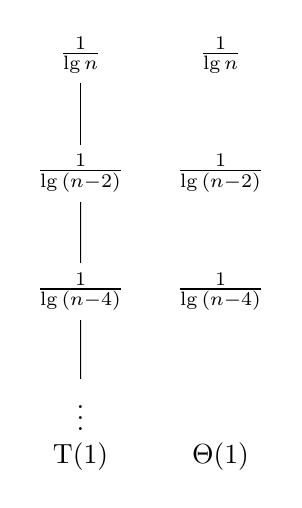
\begin{tikzpicture}

\node (root){$\frac{1}{\lg{n}}$}
    child {node {$\frac{1}{\lg{(n - 2)}}$}
        child {node {$\frac{1}{\lg{(n - 4)}}$}
            child {node {$\vdots$}[no edge from this parent]
                child {node {T(1)}}}}};

\node[right=1 of root] {$\frac{1}{\lg{n}}$}[no edge from this parent]
    child {node {$\frac{1}{\lg{(n - 2)}}$}[no edge from this parent]
        child {node {$\frac{1}{\lg{(n - 4)}}$}[no edge from this parent]
            child {node {}[no edge from this parent]
                child {node {$\Theta(1)$}}}}};
\end{tikzpicture}
\end{document}